\documentclass{beamer}
\usepackage[utf8x]{inputenc}
%\usepackage[latin1]{inputenc}
\usepackage[ngerman]{babel}
\usepackage{graphicx}
\usetheme{Warsaw}
\usecolortheme{default}
\useinnertheme{circles}
%\useoutertheme{smoothbars}
%\useoutertheme{infolines}
%\useoutertheme{miniframes}
%\useoutertheme{sidebar}
%\useoutertheme{split}
%\useoutertheme{shadow}
%\useoutertheme{smoothtree}
%\useoutertheme{tree}
%\useoutertheme{miniframes}
\usepackage{amsmath}
\usepackage{amsfonts}
\usepackage{amssymb}
\setbeamercovered{transparent}
\title{WM Tippspiel 2010}
\author{Schächterle - Heimstädt - Cuartas}
\institute[]{Hochschule Augsburg}
%\logo{\pgfimage[width=2cm,height=2cm]{bilder/logo.jpg}}
\date{\today}

\begin{document}

\frame{\titlepage}
\section[]{}
\frame{
	\frametitle{Inhaltsverzeichnis}
	\begin{columns}[c]
	\begin{column}{5cm}
		\tableofcontents[section, subsectionstyle=hide]
	\end{column}
	\begin{column}{5cm}
		\begin{figure}[htbp]
 		 \centering
			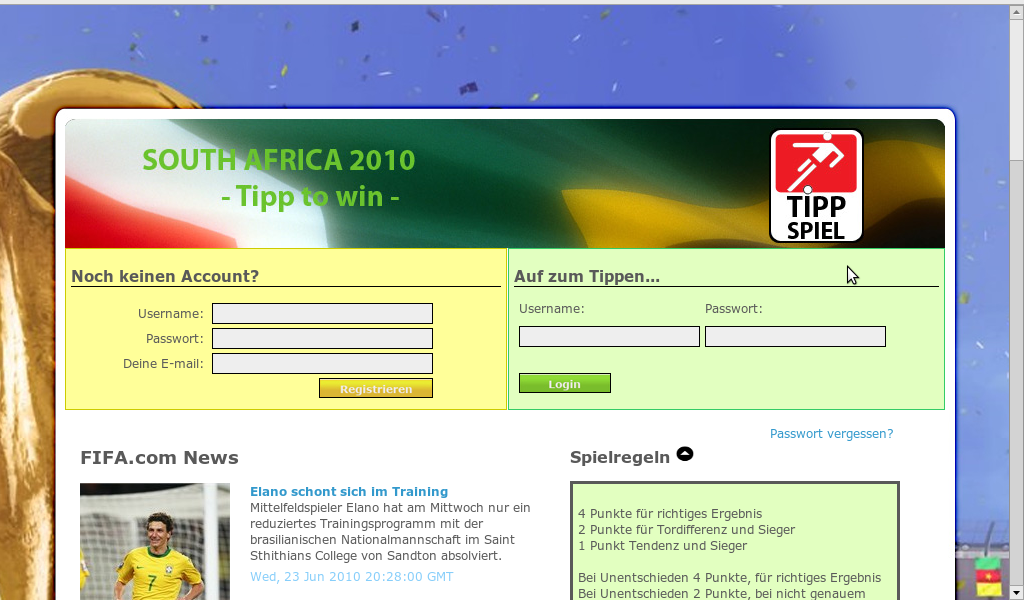
\includegraphics[width=5cm,height=4cm]{images/wmtippspiel.png}
		\end{figure}
	\end{column}
	\end{columns}
}

\section{Aufgabenstellung}
\frame{
	\frametitle{Beschreibung}
		\begin{columns}[c]
		\begin{column}{5cm}
        \begin{block}{Beschreibung}
			\begin{itemize}
				\item Fußball Tippspiel   
				\item Tipper sollen auf die Spiele der WM 2010 in Südafrika tippen   
				\item Auswertung der erzielten Punkte    
				\item Vergleich mit anderen Spielern    
				\item Einfache Benutzung    
            \end{itemize}
        \end{block}
		\end{column}
		\begin{column}{5cm}
			\begin{figure}[htbp]
 			 \centering
				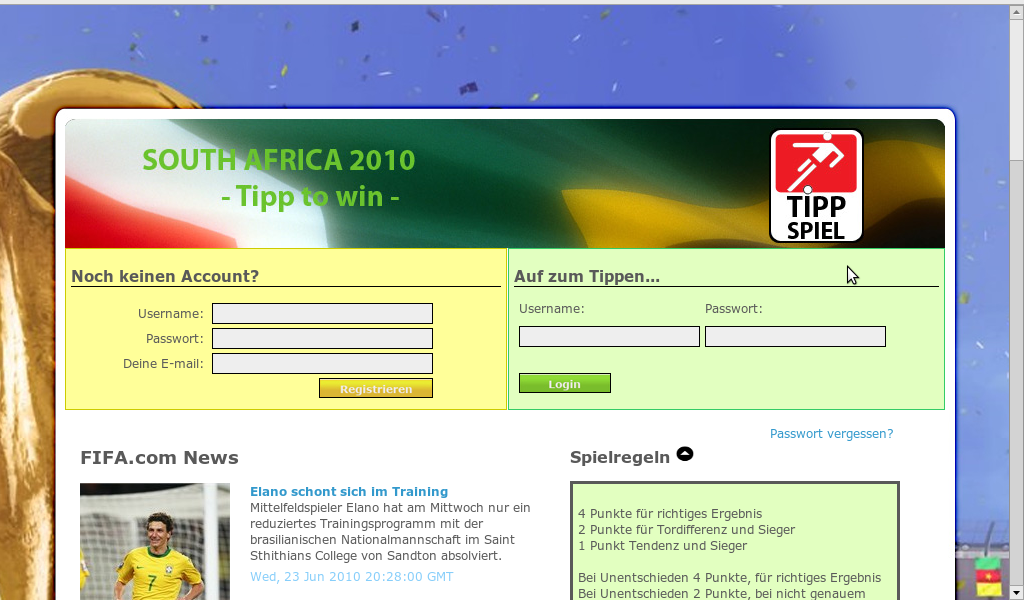
\includegraphics[width=4cm,height=3cm]{images/wmtippspiel.png}
			  \caption{WM Tippspiel}
			  \label{wmippspiel}
			\end{figure}

		\end{column}

		\end{columns}
}



\section{Technologien}
\frame{
	\frametitle{Django}
		\begin{columns}[c]
		\begin{column}{5cm}
        \begin{block}{Beschreibung}
			\begin{itemize}
				\item Nutzt MVC  
				\item OR-Mapper  
				\item URL-Dispatcher  
				\item Template Sprache  
            \end{itemize}
        \end{block}
		\end{column}
		\begin{column}{5cm}
			\begin{figure}[htbp]
 			 \centering
				
\includegraphics[width=4cm,height=3cm]{images/django.jpg}
			  \caption{django}
			  \label{Django}
			\end{figure}

		\end{column}

		\end{columns}
}

\frame{
	\frametitle{Webserver}
		\begin{columns}[c]
		\begin{column}{5cm}
        \begin{block}{Beschreibung}
			\begin{itemize}
				\item Apache  
				\item mod wsgi (Verbindung zu Django) 
				\item PostgreSQL (Produktiv) 
				\item MySQL (Entwicklung) 
            \end{itemize}
        \end{block}
		\end{column}
		\begin{column}{5cm}
			\begin{figure}[htbp]
 			 \centering
				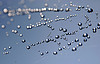
\includegraphics[width=4cm,height=3cm]{images/web.jpg}
			  \caption{Web}
			  \label{web}
			\end{figure}

		\end{column}

		\end{columns}
}


\section{Implementierung}

\frame{
	\frametitle{Blah}
		\begin{columns}[c]
		\begin{column}{5cm}
        \begin{block}{Beschreibung}
			\begin{itemize}
				\item Blah 
            \end{itemize}
        \end{block}
		\end{column}
		\begin{column}{5cm}
			\begin{figure}[htbp]
 			 \centering
				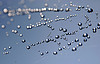
\includegraphics[width=4cm,height=3cm]{images/web.jpg}
			  \caption{Container}
			  \label{container}
			\end{figure}

		\end{column}
		\end{columns}
}

\frame{
	\frametitle{blah2}\begin{figure}[htbp]
 			 \centering
				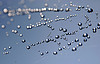
\includegraphics[width=8cm,height=6cm]{images/web.jpg}
			  \caption{Blah2}
			  \label{blah2}
			\end{figure}
}


\section{Demo}

\frame{
	\frametitle{Demo}\begin{figure}[htbp]
 			 \centering
				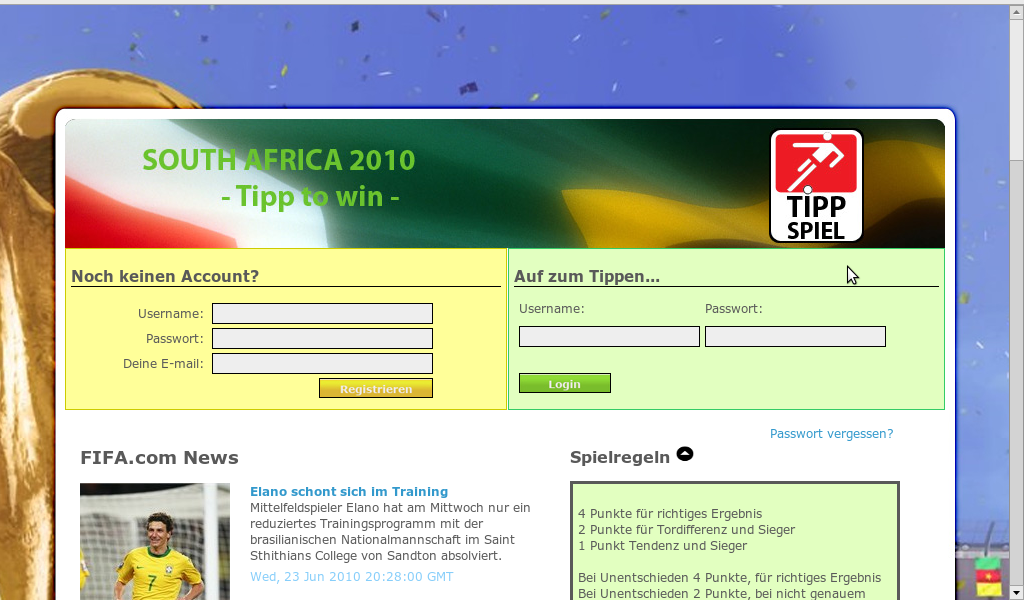
\includegraphics[width=10cm,height=4cm]{images/wmtippspiel.png}
			  \caption{Demo}
			  \label{demo}
			\end{figure}
}


\end{document}
